\chapter{Background and Literature Review}
\label{ch:literature_review}

\section{Overview of Private 5G Networks}

Private 5G networks are dedicated wireless communication systems designed to serve specific organizations, locations, or use cases. Unlike public 5G networks operated by telecom providers, private 5G networks are owned and managed by enterprises, offering greater control, customization, and security. These networks are gaining attraction due to their ability to meet the growing demands for high-speed, low-latency connectivity in various industries \cite{private5g_trends}.

Private 5G networks have several defining characteristics. They can operate on licensed, unlicensed, or shared spectrum, ensuring interference-free and reliable communication. One key capability is network slicing, which allows the creation of multiple virtualized and isolated logical networks over the same physical infrastructure, each optimized for specific services such as IoT, video surveillance, or AR/VR. Combined with ultra-low latency and high bandwidth, these features make private 5G ideal for mission-critical applications such as industrial automation, autonomous vehicles, and smart infrastructure \cite{5g_architecture_overview}.

The benefits of private 5G are widely recognized. These networks offer enhanced security by isolating traffic from public infrastructure, improved reliability and performance compared to Wi-Fi, and greater control over network policies and traffic flows. In addition, private 5G facilitates integration with legacy systems while supporting advanced technologies like AI/ML, edge computing, and massive IoT deployments \cite{5g_enterprise_benefits}.

Use cases span various sectors. In manufacturing, private 5G enables smart factories with real-time monitoring and robotics. In healthcare, it supports telemedicine and connected medical devices. Logistics and warehousing benefit from AGV coordination and inventory management, while educational institutions leverage private 5G for research and immersive learning. Smart cities deploy private 5G for public safety, traffic optimization, and infrastructure automation \cite{5g_industry_applications}.

Despite these advantages, several challenges hinder widespread adoption. The high cost of infrastructure, the complexity of deployment and orchestration, and difficulties integrating with legacy systems remain critical barriers. Resource limitations in SMEs and academic institutions further complicate deployment efforts. Finally, the lack of skilled professionals familiar with 5G, SDN, and NFV technologies represents a significant constraint \cite{5g_challenges_summary}.


\section{Overview of the Aether Platform}

Aether is a leading open-source private 5G platform developed by the Open Networking Foundation (ONF) to deliver scalable, flexible, and secure enterprise connectivity. It provides a modular, cloud-native framework for deploying and managing private 5G networks, offering advanced features such as network slicing, runtime policy control, and real-time observability \cite{aether_overview}. Aether is particularly well-suited for both enterprise deployment and academic experimentation, thanks to its Kubernetes-based architecture, open APIs, and extensible blueprint system.

\subsection*{Architecture of Aether}

Figure~\ref{fig:aether-arch} shows the high-level architecture of Aether deployed in an edge cloud environment. It highlights how SD-Core, SD-RAN, AMP, and other components interact within a cloud-native stack hosted on-premises. This architecture enables local breakout and aligns with enterprise-grade deployment requirements.

\begin{figure}[H]
    \centering
    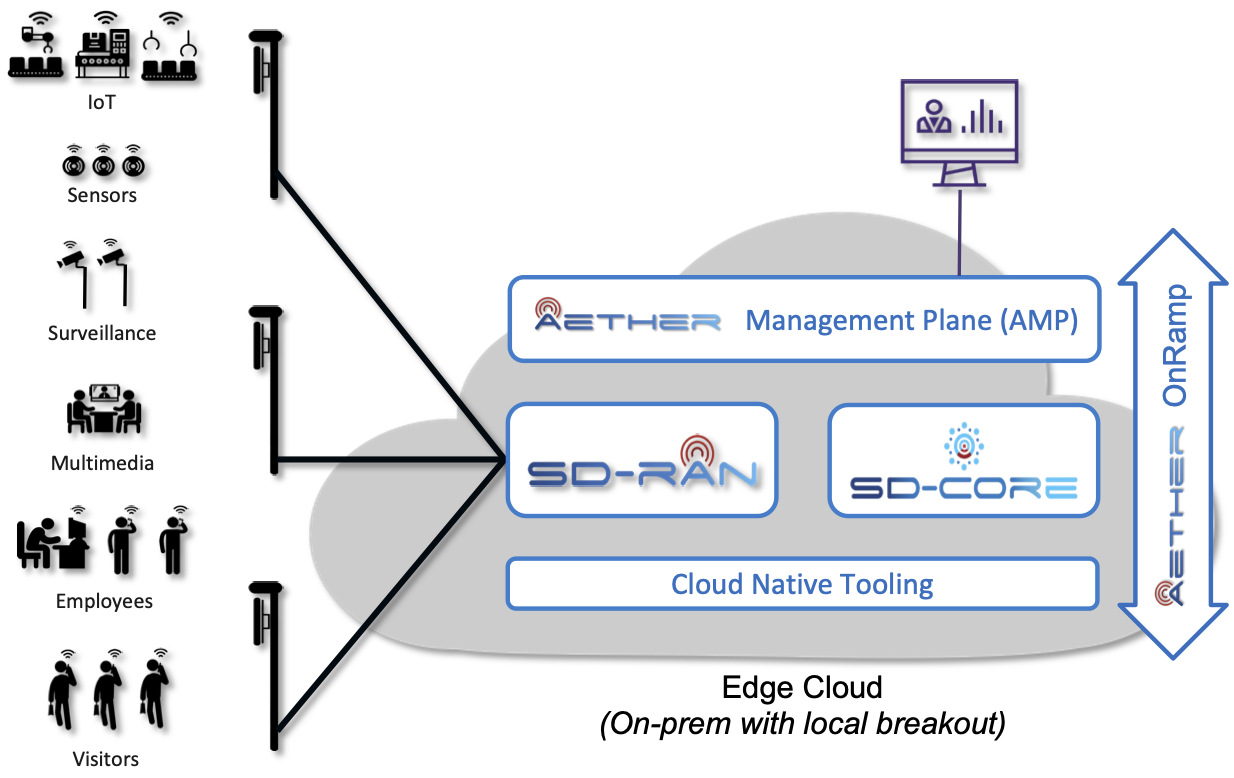
\includegraphics[width=0.95\textwidth]{Hassan_Thesis/images/Aether/Aether-Arch.png}
    \caption{High-Level Architecture of the Aether Platform \cite{aether_overview}.}
    \label{fig:aether-arch}
\end{figure}



\subsection*{Key Components of Aether}

Aether consists of several core components that integrate to provide end-to-end private 5G services:

\paragraph{SD-Core (Software-Defined Core):}

SD-Core, also known as the Aether Core, is a cloud-native mobile core designed to support 4G LTE, 5G non-standalone (NSA), and 5G standalone (SA) deployments within a unified architecture \cite{sdcore_whitepaper}. It provides a modular service-based design, aligning with 3GPP-defined principles for next-generation networks.

The control plane of SD-Core includes the Access and Mobility Management Function (AMF), Session Management Function (SMF), User Plane Function (UPF), User Data Management (UDM), and related functions—all implemented as containerized microservices. The user plane is powered by BESS (Berkeley Extensible Software Switch), enabling high-performance packet forwarding at the edge.

SD-Core exposes a rich runtime API that allows network operators and third-party systems to:
\begin{itemize}
    \item Dynamically provision and manage subscribers.
    \item Configure and apply QoS policies across network slices.
    \item Control runtime behavior of core functions (e.g., SMF, UPF).
    \item Stream telemetry data for monitoring and closed-loop automation.
\end{itemize}

This API-driven approach makes SD-Core highly suitable for edge computing environments and allows integration with intelligent applications that can dynamically influence the network.

For development and testing purposes, SD-Core includes \texttt{gNBsim}, an open-source radio access emulator. This tool enables simulation of large-scale UE attach, session establishment, and control plane signaling without requiring physical radios, making it ideal for CI/CD pipelines and lab environments \cite{sdcore_gnbsim}.

\begin{figure}[H]
    \centering
    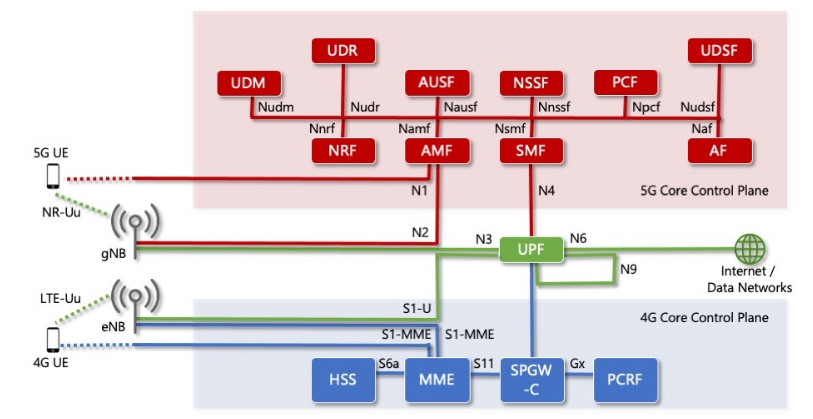
\includegraphics[width=0.9\textwidth]{Hassan_Thesis/images/Aether/SD-Core-Arch.png}
    \caption{SD-Core Architecture Overview \cite{sdcore_whitepaper}.}
    \label{fig:sdcore-arch}
\end{figure}


\paragraph{SD-RAN (Software-Defined Radio Access Network)}

SD-RAN is an O-RAN compliant, open-source Radio Access Network stack developed by the Open Networking Foundation (ONF). It implements the 7.2x functional split, separating the Distributed Unit (DU), Centralized Units for Control (CU-C), and User plane (CU-U). This split supports disaggregation and flexible deployment across edge and cloud environments.

At the heart of SD-RAN is the Near-Real Time RAN Intelligent Controller (nRT-RIC), built on the cloud-native \textmu{}ONOS platform. The nRT-RIC enables policy-based control over RAN behavior by hosting a variety of xApps, including:

\begin{itemize}
    \item \textbf{RRM xApps:} For radio resource management and traffic steering.
    \item \textbf{SON xApps:} Supporting self-optimization of network parameters.
    \item \textbf{Policy xApps:} For applying high-level business rules across the RAN.
\end{itemize}

The nRT-RIC interacts with RAN components through standardized O-RAN interfaces such as A1 (for policy control) and E2 (for real-time telemetry and control). It supports the E2SM-KPM and E2SM-RC service models for monitoring and control of key performance indicators and RAN configuration, respectively.

To enable closed-loop testing and development of xApps, SD-RAN includes \texttt{RANSIM}, a simulator capable of generating realistic radio events and performance metrics. This makes it possible to develop, test, and validate RIC behavior and xApps in a fully virtualized environment \cite{sdran_ransim}.

\begin{figure}[H]
    \centering
    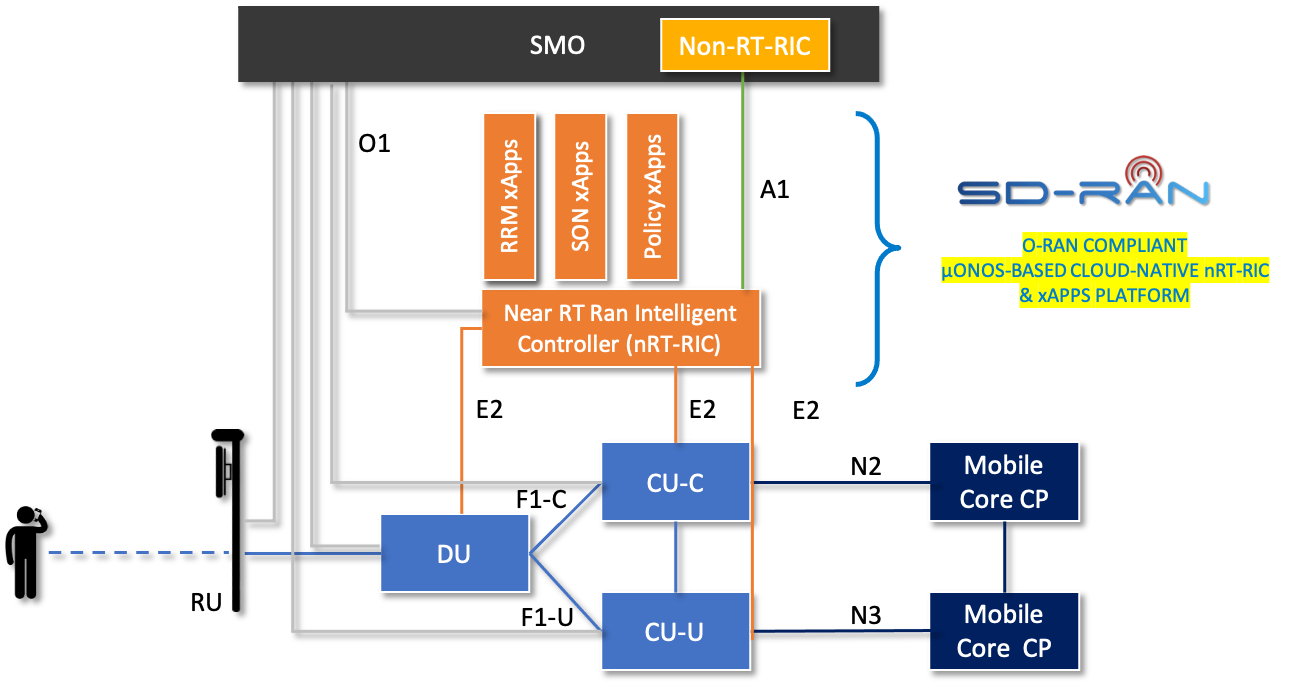
\includegraphics[width=0.95\textwidth]{Hassan_Thesis/images/Aether/SDRAN-Arch.png}
    \caption{SD-RAN Architecture Overview showing the integration of nRT-RIC with xApps, CU/DU elements, and mobile core control planes \cite{sdran_ransim}.}
    \label{fig:sdran-arch}
\end{figure}


\paragraph{AMP (Aether Management Plane):}

The Aether Management Plane (AMP) provides runtime control, monitoring, and lifecycle management functionality for the Aether platform. It operates on top of SD-Core and SD-RAN to enable dynamic configuration and observability of deployed network services. AMP comprises two principal subsystems:

\begin{itemize}
    \item \textbf{Runtime Operational Control (ROC):} Built on \textmu ONOS (a microservices-based evolution of the ONOS SDN controller), ROC exposes REST APIs and a GUI for managing network slices, user groups, policy profiles, and operational parameters at runtime.
    
    \item \textbf{Monitoring Subsystem:} This subsystem integrates with open-source monitoring tools like Prometheus, Grafana, and Rancher, and features custom dashboards for real-time visibility into Aether's operational state \cite{roc_monitoring}.
\end{itemize}

From an architectural standpoint, AMP enables closed-loop control by combining monitoring and runtime control into a unified interface for operators. Through telemetry data collection and actionable control APIs, AMP supports use cases such as dynamic QoS enforcement, resource scaling, and anomaly detection.

In addition to runtime operations, AMP also interfaces with lifecycle management systems responsible for provisioning, upgrades, and configuration versioning. These responsibilities are coordinated through a code-based pipeline where operators and developers contribute infrastructure changes via repository commits, triggering system upgrades or provisioning workflows.

Figure~\ref{fig:amp-arch} shows a simplified representation of the AMP architecture. It highlights the interactions between users, developers, and operations teams, and how those roles interface with the platform via REST APIs, provisioning pipelines, and runtime controllers.

\begin{figure}[H]
    \centering
    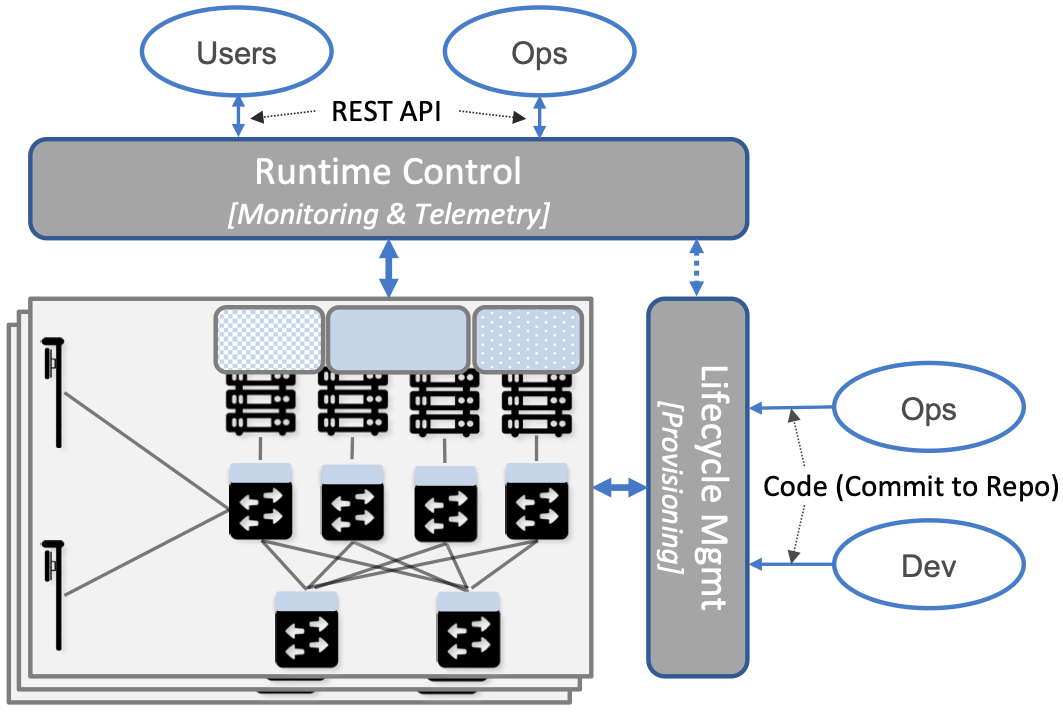
\includegraphics[width=0.95\textwidth]{Hassan_Thesis/images/Aether/Aether-Managment.png}
    \caption{Simplified architecture of Aether Management Plane, integrating runtime control (monitoring + telemetry) and lifecycle provisioning \cite{roc_monitoring}.}
    \label{fig:amp-arch}
\end{figure}


\paragraph{OnRamp:}  
Aether OnRamp simplifies deployment through pre-built infrastructure blueprints, which encapsulate a declarative configuration of the entire stack, including SD-Core, SD-RAN, and AMP. These blueprints are defined using Ansible variables, roles, and playbooks, allowing reproducible and version-controlled deployments across different environments. OnRamp supports Kubernetes-based orchestration (using RKE2) and installs all Aether subsystems as containerized applications via Helm charts \cite{onramp_docs}.




\section{Virtualization in 5G}
\label{sec:virtualization_5g}

Virtualization is a foundational pillar in modern 5G network design, enabling the shift from hardware-based appliances to software-defined, cloud-native solutions. In traditional mobile networks, core components such as the Access and Mobility Management Function (AMF), User Plane Function (UPF), and Radio Access Network (RAN) controllers were tightly coupled with proprietary hardware. With the introduction of Network Function Virtualization (NFV) and Software-Defined Networking (SDN), these functions are now implemented as software applications that can run on general-purpose servers and virtualized platforms \cite{nfv_sdn_intro}.

The 5G ecosystem leverages multiple layers of virtualization. At the infrastructure level, Virtual Machines (VMs) provide hardware isolation and compatibility across different operating systems. On top of VMs, lightweight containers such as Docker streamline the packaging and deployment of 5G components by bundling applications with their dependencies. Containers are orchestrated using Kubernetes, which has emerged as the industry standard for managing distributed, scalable applications \cite{5g_kubernetes_cnfs}. It automates deployment, scaling, networking, and lifecycle management of containerized services, making it a natural fit for dynamic 5G environments.

Virtualization introduces several benefits for 5G deployments. It improves resource utilization by enabling on-demand scaling of network functions, supports multi-tenancy and network slicing, and accelerates deployment cycles through automated CI/CD pipelines \cite{etsi_nfv}. Moreover, it allows operators to deploy private 5G networks in a variety of scenarios, ranging from public cloud to private on-premise edge clouds, offering maximum flexibility and cost-efficiency.

Despite these advantages, virtualization also presents challenges, especially in resource-constrained environments like small enterprise testbeds or academic labs. Running complex 5G stacks in single-node or dual-node VM setups can lead to CPU, memory, and storage bottlenecks \cite{5g_testbeds_virtualization}. I/O performance—particularly for telemetry and monitoring pipelines—may degrade in the absence of high-throughput hardware. Additionally, configuring multi-interface networking and maintaining inter-container communication can be technically demanding in environments with limited orchestration support. These constraints are particularly relevant to the context of this thesis, which evaluates Aether’s performance under such limitations.

The Aether platform embraces a fully virtualized, cloud-native architecture. Each of its components—SD-Core, SD-RAN, AMP, and OnRamp—is deployed as a set of containerized microservices managed by Kubernetes. Using its Ansible-based blueprint system, Aether can be instantiated on standard virtual machines without the need for specialized hardware. This design not only simplifies deployment but also enables experimentation and testing in real-world, resource-limited environments. It highlights the viability of deploying private 5G networks using open-source software and virtualization tools—a central focus of this research \cite{aether_overview}.


\newpage
\section{Related Work}
\label{sec:related_work}

The deployment of private 5G networks has gained increasing attention in both academic and industrial domains. A range of commercial and open-source platforms have emerged to support enterprise-grade 5G connectivity, with implementations spanning from public cloud environments to on-premise edge infrastructures. Existing literature has explored various architectural models, orchestration frameworks, and performance evaluations of these deployments—especially in large-scale or telecom-grade settings \cite{private5g_trends,5g_architecture_overview}.

Several research testbeds, including 5GENESIS, POWDER, and COSMOS, provide extensive infrastructures for 5G experimentation. These platforms support advanced features such as network slicing, user mobility, and RAN control experimentation, and often provide field-tested datasets. However, they typically depend on specialized hardware, dedicated spectrum, and custom orchestration systems, which may be infeasible for institutions or enterprises with limited technical and financial resources \cite{5g_testbeds_overview}.

Virtualization is widely regarded as a cornerstone of 5G architecture. Numerous studies have investigated the role of NFV and SDN in enabling scalable, cloud-native deployments of core and RAN functions. Kubernetes-based orchestration of containerized network functions (CNFs) has become a popular research focus due to its flexibility and extensibility in managing dynamic workloads \cite{5g_kubernetes_cnfs,etsi_nfv}. Nevertheless, most of these studies assume access to robust, resource-rich infrastructure, which does not reflect the constraints of small-scale labs or academic testbeds.

Among open-source 5G platforms, the Aether project stands out as a modular, cloud-native solution for private 5G. Although its architecture and potential use cases have been described in technical documentation and white papers \cite{aether_overview,sdcore_whitepaper}, there is limited academic literature evaluating Aether in constrained or resource-limited settings. In particular, empirical studies examining multi-blueprint deployments, runtime control using ROC, and the use of monitoring tools like Prometheus and Grafana in small-scale environments remain sparse.

This thesis addresses these gaps by evaluating Aether’s deployment in VM-based environments with limited resources. It investigates the system’s performance, reproducibility, and usability in settings aligned with academic and enterprise edge use cases—thereby contributing new insights to the growing body of research on private 5G platforms.



\section{Research Gaps}

The deployment of private 5G solutions—particularly platforms like Aether—has gained significant momentum due to their potential to deliver secure, flexible, and high-performance connectivity in enterprise and academic environments. However, despite advancements in this domain, several key gaps remain in the existing literature:

\begin{enumerate}
    \item \textbf{Lack of VM-Based Deployment Evaluations} \\
    Existing studies predominantly focus on cloud-native or containerized deployments, typically leveraging high-resource clusters or public cloud infrastructures. In contrast, there is limited research on deploying and evaluating private 5G platforms like Aether within \textit{virtualized environments using constrained hardware}, such as single-node or dual-node VM setups. This limitation is especially relevant for educational institutions and small enterprises that depend on general-purpose computing infrastructure for experimentation and learning environments.

    \item \textbf{Insufficient Analysis of Multi-Blueprint Scenarios} \\
    Aether supports multi-blueprint deployments, including components such as Runtime Operational Control (ROC), multiple UPFs, and monitoring dashboards. However, \textit{empirical studies investigating the interaction, performance, and scalability} of these blueprints—particularly in isolated or resource-limited testbeds—are scarce. Without such evaluations, the real-world applicability and performance trade-offs of complex blueprint combinations remain unclear.

    \item \textbf{Minimal Stress-Testing in Resource-Constrained Systems} \\
    While some works explore 5G core network performance under ideal conditions, few attempt to \textit{stress-test private 5G deployments on limited resources}, especially using simulators such as gNBsim or UERANSIM. These tools can expose system bottlenecks related to CPU, memory, and I/O in VM environments, yet this aspect remains largely underexplored.

    \item \textbf{Underrepresentation of Educational and Reproducible Testbeds} \\
    Despite the open-source nature of Aether, its potential as an educational platform is not well documented. There is a noticeable gap in the literature regarding the design and deployment of \textit{reproducible, VM-based testbeds} that can be used for teaching, rapid prototyping, or hands-on training. Addressing this can significantly improve accessibility to 5G research and training in university settings.

    \item \textbf{Limited Insights into Real-Time Control and Monitoring Tools in Small-Scale Deployments} \\
    Tools like Aether ROC and Prometheus-Grafana are essential for runtime control and observability in 5G networks. However, their \textit{integration, usability, and performance under stress in small-scale VM testbeds} are rarely analyzed. This limits our understanding of how dynamic policies, monitoring, and network slicing behave outside large-scale, cloud-optimized setups.
\end{enumerate}

By addressing these research gaps, this study contributes to the practical understanding and reproducibility of enterprise-facing private 5G deployments in virtualized environments. The insights gained aim to inform future implementations, both in academic labs and in real-world enterprise settings.

\section{Chapter Summary and Motivation}
\label{sec:chapter2_summary}

This chapter presented a comprehensive background on private 5G networks, focusing on their key architectural features, deployment models, and the virtualization technologies that enable flexible, scalable implementations. It also explored the Aether platform—an open-source, cloud-native private 5G solution—and analyzed its core components, including SD-Core, SD-RAN, AMP, and OnRamp. A review of related research highlighted ongoing efforts in 5G deployment and experimentation, particularly within large-scale cloud or testbed environments.

Despite these advancements, several important research gaps persist, particularly around the deployment and evaluation of private 5G solutions in constrained virtualized environments. These include the limited availability of VM-based testbeds, lack of empirical analysis of multi-blueprint deployments, and underrepresentation of educational or reproducible Aether setups. This thesis addresses these gaps by studying Aether’s behavior in resource-limited VM setups, with a focus on reproducibility, runtime control, and performance stress-testing.

The next chapter presents the methodology, experimental testbed, and blueprint configurations used to evaluate these research challenges in a controlled, virtualized setting.
